%% -*- coding:utf-8 -*-
\documentclass[ number=??
			   ,series=lnls,
			   ,output=long    % long|short|inprep              
			   %,blackandwhite
			   %,smallfont
			   ,draftmode  
			  ]{langsci}                          

          
\hypersetup{pdfdisplaydoctitle=true}

\usepackage{xspace}
\newcommand{\latex}{\LaTeX\xspace}

% just for the XeLaTeX logo
\usepackage{dtklogos}\newcommand{\xelatex}{\XeLaTeX\xspace}
\newcommand{\bibtex}{\BibTeX\xspace}

\newcommand{\lsp}{Language Science Press\xspace}

\usepackage{lsp-makros}

\usepackage{german}\selectlanguage{USenglish}
% AVMs

\usepackage{styles/avm}
\avmfont{\sc} 
\avmvalfont{\it}
      
% OT pointing hand
\usepackage{pifont}
\newcommand{\hand}{\ding{43}}

% OT tableaux                                                
\usepackage{pstricks,colortab}   


\usepackage{tikz-qtree}
% has strange side effects
%\tikzset{every tree node/.style={align=left, anchor=north}}
\tikzset{every roof node/.append style={inner sep=0.1pt,text height=2ex,text depth=0.3ex}}

 
\usepackage{lipsum}  

% Chinese
\usepackage[indentfirst=false]{xeCJK}
\setCJKmainfont{SimSun}

% bidirectional text and support for Arabic/Persian
%% \usepackage{fontspec}
\newfontfamily\Parsifont[Script=Arabic]{XB Niloofar}
%\usepackage{bidi}
%\newcommand{\PRL}[1]{\RL{\Parsifont #1}}


\usepackage{lsp-gb4e}

\title{How to Write a Book for Language Science Press}  
\subtitle{Guidelines for Authors and \latex Recommendations}
\BackTitle{How to Write a Book for Language Science Press}
\BackBody{This book contains the guidelines for Language Science Press authors. For those who want
  to help keeping the production costs low and therefore decided to use \latex it also contains
  descriptions of packages that can be used for typesetting trees, Attribute Value Matrices, OT-tableaux, Categorial
  Grammar proofs, LFG analyses, and much more. The setup of typesetting script with special fonts as
  for instance right to left scripts like Arabic is explained. The \latex chapter also contains sections
  concerning the efficient workflow in professional typesetting environments using \latex.

Stefan Müller is an experience \latex user who has typeset four published books and several book
manuscripts and journal articles.
}

\dedication{This book is dedicated to everybody who cannot afford buying books by profit oriented publishers.}

\author{Stefan Müller}



\makeatletter
\def\verbatim@font{\scriptsize\ttfamily}
\makeatother
         
\begin{document}               
         
                                                                           
                                  
\maketitle                

\frontmatter

\chapter*{Vorwort}

\lipsum[3-10]  

\section*{Acknowledgements}

%% David Reitter danke ich für die \LaTeX"=Makros für Combinatorial
%% Categorial Grammar, Mary Dalrymple und Jonas Kuhn für die LFG"=Makros und Beispielstrukturen, und
%% Laura Kallmeyer für die \LaTeX"=Quelltexte der meisten TAG"=Analysen. Ohne diese
%% Originalmakros/-texte wären die Darstellungen in den jeweiligen Kapiteln sicher nicht halb so schön
%% geworden. 

This book is typeset with \LaTeX. We thank the \LaTeX{} developers for their work and the members of the German \textit{German
  Language TeX Users Group Communication List} and those replying at \url{http://tex.stackexchange.com} for many usefull hints and suggestions.


\bigskip

\noindent
Berlin, \today\hfill Stefan Müller


\tableofcontents      

\mainmatter         

%% -*- coding:utf-8 -*-
\chapter{Style rules for authors}

Authors can submit books after registering as an author at
\url{http://langsci-press.org/user/register}. \lsp only publishes books that are assigned to a
series. It is suggested that authors contact the series editor informally before an official submission.
The submission has to be in PDF format to make proper
reviewing (reference to page numbers) possible. The first submission does not have to correspond to
the format specification that is outlined in this chapter, but if it does this is good since it
enables series editors to get some idea about the length of the book and so on. If authors submit an
almost final version in the proper layout, this speeds up production, since comments on form can be
provided in the first reviewing steps.


The following sections describe the layout of various items that play a role in typesetting. Many of
these things are covered automatically by the Word Template\footnote{
\url{https://github.com/langsci/word}, 19.02.2014.
} or by our \latex classes\footnote{
\url{https://github.com/langsci/latex}, 19.02.2014.
}. Authors who start a new book project are strongly recommended to use \latex from the very beginning.


\section{Front matter}
The front matter of \lsp books is structured as follows
\begin{itemize}
 \item optional dedication
 \item obligatory table of contents 
 \item obligatory Notes on contributors (only in edited volumes)
 \item optional notational conventions
 \item optional acknowledgements
 \item optional preface
 \item optional list of abbreviations
 \item no lists of figures or lists of tables!
\end{itemize}

\section{Back matter}
The back matter is structured as follows:

\begin{itemize}
 \item optional Appendix A
 \item optional Appendix B etc
 \item optional further appendices
 \item obligatory Bibliography
 \item obligatory Author index
 \item optional Language index (advisable if the book talks about a larger number of languages)
 \item obligatory Subject index
 
\end{itemize}


\section{Chapters}

Every book is divided into consecutively numbered chapters. In addition to chapters, a book may also
group chapters into parts (numbered I, II, III). %Chapter numbering is not restarted within parts.




\section{Sections and headings}

All sections (= parts of chapters) have headings and are numbered. Authors may use structures with up to
six levels, i.e. there may be a section with the number 1.2.3.4.5.6.\footnote{
  See page~\pageref{sec-Chinese} for an actual use of subsubsections.%
} However, such elaborated
structures may be difficult for the readers, so there should be a good motivation for going beyond
three or four levels.

Sections and subsections must be minimally two and must be exhaustive. This means that all text in a chapter
must belong to some section, all text within a section must belong to some subsection and so on. A
short intro paragraph is allowed by way of exception, as in the current Section 3 (see the intro
paragraph above Section 3.1).\todo{würde ich nicht erlauben SN}

Please do not change the capitalization of words when they are used in titles. 
% Please write the headings of chapters and sections without special capitalization.
This also applies
to the title (and subtitle) of the book itself and to the bibliographical references. Language
Science Press never uses special capitalization.
% , as it potentially introduces ambiguity, and there are no clear rules for special capitalization in English anyway.

\section{Italics, small caps, and punctuation marks}

\textbf{Boldface} is generally restricted to section headings.
\textit{Italics} are used for the following purposes:
\begin{enumerate}
\item for all object-language forms that are cited within the text or in set-off examples (e.g. in (2) and (4) below), unless they are written in IPA or otherwise in the context of the discussion of sounds;
\item  when a technical term is referred to, e.g. ``the term \textit{quotative} is not appropriate here'', or ``I call this construction \textit{quotative}''. In such contexts, English technical terms are thus treated like object-language forms;
\item for emphasis of a particular word that is not a technical term (``This is possible here, but \textit{only} here'').
\textsc{Small caps} are used for highlighting important terms on first mention, e.g.
\end{enumerate}
\ea
On this basis, the two main alignment types, namely \textsc{nominative-accusative} and \textsc{ergative-absolutive}, are distinguished.
\z

Small caps are also used for category abbreviations in interlinear glossing, and they may be used to indicate stress or focusing in example sentences:

\ea 
John called Mary a Republican and then \textsc{she} insulted \textsc{him}.
\z


% To emphasize terms, please use \emph{italics}. Boldface should be avoided if
% possible. New terms should be set in {\sc small caps}.
% EN-dashes are used for ranges (e.g.\ 1985–1995).

Double quotation marks are generally used for distancing, in particular in the following situations:
\begin{enumerate}
 \item  when a passage from another work is cited in the text (e.g. According to Takahashi (2009: 33), ``quotatives were never used in subordinate clauses in Old Japanese''); but block quotations do not have quotation marks;
\item when a technical term is mentioned that the author does not want to adopt, but wants to mention, e.g.

\ea
This is sometimes called ``pseudo-conservatism'', but I will not use this term here, as it could lead
to confusion.
\z


\end{enumerate}


Single quotation marks are used exclusively for linguistic meanings, as in the following:
\ea
Latin \textit{habere} `have' is not cognate with Old English \textit{hafian} `have'.
\z

\section{Glossed examples}

Please gloss all example sentences from languages other than English and provide them with idiomatic translations. The glossing should be done according
to the Leipzig Glossing Rules. 
If you need special abbreviations that are not defined by the Leipzig Glossing Rules, put them in a table in a special section with abbreviations immediately before the first chapter of a monograph. In the case of an edited volume, the lists of abbreviations should be placed immediately before the references of the individual chapers.

The formatting of example sentences in the typological series follows the format that is used by the World Atlas of Language Structures (Haspelmath et al. 2005): If there is just one example sentence for an example number, the language name follows the example number directly, as in (\ref{ex-typology}); it may be followed by the reference.

{\def\exfont{\normalsize\itshape}
\ea\label{ex-typology}
{\rm Mising\il{Mising} \citep[69]{Prasad91a}}\\
\gll azɔ́në dɔ́luŋ\\
     small village\\ 
\glt `a small village' 
\z


If there are two sub-examples for a single example number, the example heading may have scope over both of them:

\ea
{\rm Zulu}{(Poulos \& Bosch 1997: 19; 63)}
\ea
\gll Shay-a		inja!\\
hit-\textsc{imp.2sg}	dog\\
\glt `Hit the dog!'
\ex
\gll	Mus-a	uku-shay-a	inga! \\
	\textsc{neg.imp.aux-2sg}	\textsc{inf}-hit-\textsc{inf}	dog \\
\glt		`Do not hit the dog!'	
\z
\z

If two examples with different numbers belong to the same language, the language name is repeated only if the identity of the language is not clear from the context. If an example consists of several sub-examples from different languages, the language name and references follow the letters, as in (4):
(\mex{1}):

\eal
\ex {\rm Apatani\il{Apanti} \citep[23]{Abraham85a}}\\
\gll aki atu\\ 
     dog small\\ 
\glt ‘the small dog’ 
\ex {\rm Temiar\il{Temiar} \citep[155]{Benjamin76a}}\\ 
\gll dēk mənūʔ\\
     house big\\
\glt ‘big house’ 
\zl
}

\section{Figures and tables}

Figures and tables should come with a caption. Captions are set below figures and above tables. Like headings, the captions should not use special capitalization. 
Figures and tables are numbered. The number should consist of the chapter number and a number that starts with one for every new chapter. Figures and tables are counted separately. Figure 3.1 is an example of a figure and Table 3.1 is an example of a table.


The number should consist of the chapter number and a number that starts with 1 for every new chapter. There has to be one counter for figures and another one for tables. Figure~\vref{fig-example-fig-the-dog-barks} is an example of a figure and Table~\vref{tab-example-croft} is an example of a table.

\begin{figure}[htbp]
\centerline{%
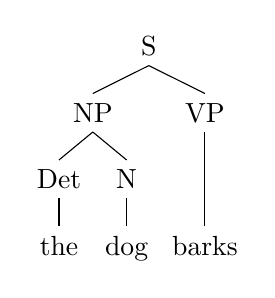
\begin{tikzpicture}
\tikzset{level 1+/.style={level distance=2\baselineskip}}
\tikzset{frontier/.style={distance from root=6\baselineskip}}
\Tree[.S
       [.NP 
         [.Det the ]
         [.N   dog ] ]
       [.VP barks ] ]
\end{tikzpicture}
}
\caption{\label{fig-example-fig-the-dog-barks}An example of a figure: Analysis of the sentence \emph{The dog barks.}}
\end{figure}

\begin{table}[htbp]
\caption{\label{tab-example-croft}An example of a table taken from \citew[214]{Croft2003a}}
\centerline{
\begin{tabularx}{\textwidth}{llX}\hline\hline
          & Low categoriality unit      & Unit with wich it clusters\\\hline
`Noun'    & low referentiality NP       & forgrounded verb\\
          & attached body part noun     & forgrounded verb\\
          & anaphoric NP                & forgrounded verb, emphasized element\\
`Verb'    & tense/aspect/mood auxiliary & forgrounded verb\\ 
\hline\hline
\end{tabularx}
}
\end{table}

\section{Footnotes}

Notes are footnotes rather than endnotes. Footnote numbers go to the end of the clause after punctuation
unless they refer to a specific word or phrase.\footnote{
  This is an example of a footnote that refers to the whole clause.
}

Footnote numbers should not be used in tables or figures\footnote{
  This is a footnote that refers to the word \emph{figures}. 
} but should be attached to the text preceding or following them.

\inlinetodostefan{Martin: [COMMENT: Manchmal braucht man solche Tabellen-internen Fußnoten; dann verwendet man manchmal Buchstaben a, b, c als Fußnotenzeichen]}


\section{Quotations}

If long passages are quoted, they should be indented and the quote should be followed by the exact reference. Use the quotation environment \latex provides:
\begin{quotation}
Precisely constructed models for linguistic structure can play an
important role, both negative and positive, in the process of discovery 
itself. By pushing a precise but inadequate formulation to
an unacceptable conclusion, we can often expose the exact source
of this inadequacy and, consequently, gain a deeper understanding
of the linguistic data.
\citep[5]{Chomsky57a}
\end{quotation}
%
Short passages should be quoted inline using quotes: \citet[5]{Chomsky57a} stated that ``[o]bscure
  and intuition-bound notions can neither lead to absurd conclusions nor provide new and
correct ones''.

If you quote text that is not in the language of the book provide a translation. Short quotes should
be translated inline, long quotes should be translated in a footnote.

\section{Cross-references in the text}

Please use the cross-referencing mechanisms of your text editing/type setting software. Using such
cross-referencing mechanisms is less error-prone when you shift text blocks around and in addition
all these cross-references will be turned into hyperlinks between document parts, which makes the
final documents much more useful.

If you have numbered example sentence, please start with (1) for every new chapter.
%%
%% Alternatively, you may put the chapter number in front of the example number (thus starting with (7.1), (7.2), ... in chapter 7, for example).
%% [COMMENT: Bei Grammatiken ist es durchaus üblich, dass alle Beispiele im Buch durchnummeriert werden. Auch in Rießlers Arbeit sind die Beispiele komplett durchnummeriert. Ich bin mir nicht sicher, wie wichtig diese Regelung ist, und ob wir nicht Volldurchnummerierung auch erlauben sollten.]

Please use capitals if you refer to numbered chapters, sections, tables, figure, or footnotes: \emph{As we have shown in
  Section~3.1}, \emph{As Figure~3.5 shows}. Do not capitalize without a number: \emph{In the
  following section we will discuss}.
Depending on the series and the langauge the book is published in authors may also use the § sign
instead of the word \emph{Section}. So the above sentence would read: \emph{As we have shown in
  §3.1}.

\section{Citations and references}
\label{sec-references-authors}

A citation is author-year information (optionally with page number or other more detailed information) in the text. A bibliographical reference is metadata about a work that is cited.

If books or larger articles are cited for a smaller point, exact page numbers should be provided. This is a good service to the readers, and it is also good for
authors since it helps them to keep track of their source and enables them to find and reread the
referenced passages and it is a good service to the readers.

For references in the bibliography, we use the \emph{Unified Style Sheet for Linguistics},\footnote{\url{http://celxj.org/downloads/UnifiedStyleSheet.pdf}}. The \bibtex file is contained in the \latex
classes that are used for typesetting \lsp books. 
Please deliver a \bibtex file with all your references together with your submissions. 
\bibtex can be exported from all common bibliography tools (We recommend BibDesk for the Mac and JabRef for all other platforms). 
Please make sure that all \bibtex fields are complete. %what is the reference of  `all'? each and every imaginable bibtexfield?
Please provide all first and last names of all authors and editors. Do not use et~al. in the Bibtex file; this will be generated automatically when inserted.
For bipartite family names like ``von Stechow'', ``Van Eynde'', and ``de Hoop'' make sure that these
family names are contained in curly brackets. These authors will then be cited as
\citet{VanEynde2006a} and \citet{vonStechow84a}. Note that Dutch names like ``de Hoop'' are not treated differently from other surnames.

The references in your \bibtex file will automatically be correctly typeset. So, provided the
\bibtex file is correct, authors do not have to worry about this. But there are some things to
observe in the main text. Please cite as shown in Table~\ref{tab-citation}.

\begin{table}[htbp]
\caption{\label{tab-citation}Citation style for \lsp}
\centerline{%
\begin{tabular}{lp{9cm}}\hline\hline
citation type & example\\\hline
author & As \citet[215]{MZ85a} have shown\\
       & As \citet[215]{MZ85a} and \citet{Bloomfield33a} have shown\\
work   & As was shown in \citew[215]{Saussure16a}, this is a problem for theories that \ldots\\
work   & This is not true \citep{Saussure16a,Bloomfield33a}.\\\hline\hline
\end{tabular}
}
\end{table}
\nocite{Bresnan82b}% something with an editor.

Citations consist of author name plus year number in parentheses (with page number or other information). There is no comma between the author name and the year number. If a citation is itself in parentheses, the parentheses around the year number are omitted (unless there is a fairly long text in the parentheses, in addition to the citation).

%% Table~\ref{tab-various-publication-types} provides examples for different publication types (book,
%% journal article, paper in an edited volume, and so on). Please refer to the bibliography at the end
%% of this book to see how the respective items are formated.

If you have an enumeration of references in the text as in \emph{As X, Y, and Z have shown}, please use
the normal punctuation of the respective language rather than special markup like `;'.

If you refer to regions in a text, for instance 111--112, please do not use 111f.\ or 111ff.\ but provide the
full information. 

\noindent
\inlinetodostefan{Say something about decapitalization. \url{http://tex.stackexchange.com/a/140071/12092}}

\section{Special terms}

If you refer to special terms, please use italics as in ``I 
use the term \emph{nominative} for \ldots



\section{Punctuation}
Please use punctuation consistently. 
If you use initial adverbial clauses, please use commas: When referring to such nominatives, I use {\ldots}.
EN-dashes are used for ranges (e.g. 1985–1995).

\section{Academic \emph{we}}

Monographs and articles that are authored by a single author should use the pronoun \emph{I} rather
than \emph{we} as in ``As I have shown in Section~3''.	

\section{Special guidelines for edited volumes}


Some special rules apply to the chapter of edited volumes:
\begin{itemize}
\item Each paper has its own list of references (unnumbered section labeled References).
% \item Each paper should start with a short abstract
\item A paper may have a special unnumbered section Acknowledgements just after the last numbered section. This is preferable to putting the acknowledgements into the footnotes.
\item A paper may have a special unnumbered section Abbreviations (or similar) just before the References. This is strongly preferred to listing the abbreviations in a footnote.
\item Chapter numbers should not be used in numbering tables and figures within such chapters.
\end{itemize}


\section{Checklist}

The following is a general checklist for authors. Author who use \latex should also consult the
checklist for advanced authors/typesetters in Section~\ref{sec-check-typesetters}.

\section{Other}

Running heads:
\begin{itemize}
\item Monographs
left-hand side: chapter number and chapter heading 
right-hand side: section number and section heading
\item Edited volumes:
left-hand side: author name
right-hand side: (chapter number and) chapter name
\end{itemize}


%% -*- coding:utf-8 -*-
\chapter{\LaTeX}

\section{Installation of the \texttt{langsci} Class}

The \latex class for typesetting Language Science Press books was developed by Timm Lichte with
help be Berthold Crysmann and me. It can be downloded from the GitHUB repository at: \url{https://github.com/langsci/latex}

Place all files and subdirectories from this repository into your local working directory (for
advanced installations see Section~\ref{sec-advanced-latex-installation}).

\section{Using the \texttt{langsci} Class}

Once you installed the classes in your system, you may look at the file \texttt{test.tex} to see how
a book can be typeset. The code of this book is available in the directory \texttt{Guidelines}. Once
you set up your \latex files you can compile them by calling 
\begin{verbatim}
xelatex yourfilename.tex
\end{verbatim}


\section{Workflow}

\subsection{Compiling the Document}

\subsection{Makefiles}

\subsection{Using Includes}


\section{Document Structure}


\section{Packages specific for Linguistics}

\subsection{Glossed Examples}


\subsection{\texttt{jambox}}


The package \texttt{jambox} can be used to provide information about the language of an example or
about a certain other aspect to be highlighted.
\settowidth\jamwidth{VSO}
\eal
\ex[]{
\gll Ingrid kiel-et il-mazzit-a.\\
     Ingrid eat-3fsg def-black.pudding-fsg\\ \jambox{(SVO)}
\glt `Ingread ate black pudding.'
}
\ex[]{
Kielet il-mazzita Ingrid. \jambox{(VOS)}
}
\ex[*]{
Kielet Ingrid il-mazzita. \jambox{(VSO)}
}
\ex[]{\label{ex-sov}
Ingrid il-mazzita kielet. \jambox{(SOV)}
}
\ex[]{\label{ex-osv}
Il-mazzita Ingrid kielet. \jambox{(OSV)}
}
\ex[]{
Il-mazzita kielet Ingrid. \jambox{(OVS)}
}
\zl

The call of \verb+\jambox+ has to follow the linebreak after the gloss:
\begin{verbatim}
\ex[]{
\gll Ingrid kiel-et il-mazzit-a.\\
     Ingrid eat-3fsg def-black.pudding-fsg\\ \jambox{(SVO)}
\glt `Ingread ate black pudding.'
}
\end{verbatim}
The distance from the right margin can be specified by passing the largest object to be placed in a
jambox to \verb+\settowidth+:

\eal
\settowidth\jamwidth{(German)}
\ex The man reads the book.    \jambox{(English)}
\ex Manden læser bogen.        \jambox{(Danish)}
\ex Der Mann liest das Buch.   \jambox{(German)}
\zl

\begin{verbatim}
\eal
\settowidth\jamwidth{(German)}
\ex The man reads the book.    \jambox{(English)}
\ex Manden læser bogen.        \jambox{(Danish)}
\ex Der Mann liest das Buch.   \jambox{(German)}
\zl
\end{verbatim}

\subsection{AVMs}

  \begin{avm}
    {\it word\/} $\rightarrow$
    \[morphs & $\@{e_1}\bigcirc\cdots\bigcirc\@{e_n}$\\
    morsyn & \@0 $(\@{m_1}\uplus\cdots\uplus\@{m_n})$\\
    rules & \< \[morphs & \@{e_1}\\mud & \@{m_1}\\ morsyn & \@0\],\ldots,
    \[morphs & \@{e_n}\\mud & \@{m_n}\\ morsyn & \@0\] \>
    \]
  \end{avm}

\subsection{Trees}

\subsection{OT Tableaux}


\begin{tabular}
       {|lc|c|c|c|}\hline   
      & \textbf{Input}  & Cnstrnt 1  &  Cnstrnt 2& Cnstrnt 3\\ \hline\hline
      & candidate 1     & *!         &           &          \\ \hline
      & candidate 2     &            &  *        &          \\ \hline
\hand & candidate 3     &            &           &  *       \\ \hline
\end{tabular}

\begin{fitverb}
\begin{tabular}
       {|lc|c|c|c|}\hline   
      & \textbf{Input}  & Cnstrnt 1  &  Cnstrnt 2& Cnstrnt 3\\ \hline\hline
      & candidate 1     & *!         &           &          \\ \hline
      & candidate 2     &            &  *        &          \\ \hline
\hand & candidate 3     &            &           &  *       \\ \hline
\end{tabular}
\end{fitverb}

\verb+\hand+ ist wie folgt definiert:

\begin{verbatim}
\usepackage{pifont}
\newcommand{\hand}{\ding{43}}
\end{verbatim}
 


\begin{tabular*}{0.95\textwidth}
    {@{\extracolsep{\fill}}|rl||c|c|c|}\hline   
      & \textbf{Input} & Constraint 1 & Constraint 2 & Constraint 3 \\ \hline\hline
      & candidate 1    & *!           &              &              \\ \hline
      & candidate 2    &              &  *           &              \\ \hline
\hand & candidate 3    &              &              &  *           \\ \hline
\end{tabular*}

\begin{fitverb}
\begin{tabular*}{0.95\textwidth}
    {@{\extracolsep{\fill}}|rl||c|c|c|}\hline   
      & \textbf{Input} & Constraint 1 & Constraint 2 & Constraint 3 \\ \hline\hline
      & candidate 1    & *!           &              &              \\ \hline
      & candidate 2    &              &  *           &              \\ \hline
\hand & candidate 3    &              &              &  *           \\ \hline
\end{tabular*}
\end{fitverb}

\begin{tabular}[t]{r|c|c|c|}
\cline{2-4}
      & /qi/  & qi    & qi         \\
\LCC 
      &       &       & \lightgray \\ \cline{2-4}
\hand & [qi]  &       & *          \\ \cline{2-4}
      & [*qi] & *!    &            \\ \cline{2-4}
\ECC
\end{tabular}


\begin{verbatim}
\usepackage{pstricks,colortab}

\begin{tabular}[t]{r|c|c|c|}
\cline{2-4}
      & /qi/  & qi    & qi         \\
\LCC 
      &       &       & \lightgray \\ \cline{2-4}
\hand & [qi]  &       & *          \\ \cline{2-4}
      & [*qi] & *!    &            \\ \cline{2-4}
\ECC
\end{tabular}
\end{verbatim}


\begin{tabular}{|l||c|c|} \hline
          &VO          &OV         \\ \hline\hline
\LCC
          &            &\lightgray \\ \hline
prefixing &Tagalog     &Ma'a       \\ \hline
\ECC
\LCC
           &\lightgray &            \\ \hline
suffixing  &Kwakwala   &Japanese    \\ \hline
\ECC
\end{tabular}

\begin{verbatim}
\begin{tabular}{|l||c|c|} \hline
          &VO          &OV         \\ \hline\hline
\LCC
          &            &\lightgray \\ \hline
prefixing &Tagalog     &Ma'a       \\ \hline
\ECC
\LCC
           &\lightgray &            \\ \hline
suffixing  &Kwakwala   &Japanese    \\ \hline
\ECC
\end{tabular}
\end{verbatim}




\subsection{Font Issues and Right to Left Scripts}

Since we are using \xelatex, all fonts that are installed in the cannonical font directories can be
used. We are using the font \texttt{Linux Libertine}, which is unicode-based and contains a lot of
the characters linguists want to use.

\subsubsection{Chinese}


\ea
\glll 狗       叫     了。\\
      gou3     jiao4   le\\
      dog      bark    ASP/CRS\\
\glt `The dog is barking.'/`The dogs are barking.'
\z

\begin{verbatim}
\usepackage[indentfirst=false]{xeCJK}
\setCJKmainfont{SimSun}

\ea
\glll 狗       叫     了。\\
      gou3     jiao4   le\\
      dog      bark    ASP/CRS\\
\glt `The dog is barking.'/`The dogs are barking.'
\z
\end{verbatim}


\subsubsection{Arabic Script}



\ea
\PRL{او مرد را دوست نخواهد داشت.}\\
 \gll   U mard rā dust naxāhad dāšt.\\
   He/she man {\sc dom} friend {\sc neg}.want have\\
\glt `He/she will not love the man.'
\z

%\begin{rtlverbatim}
%\usepackage{fontspec}
\begin{verbatim}
\newfontfamily\Parsifont[Script=Arabic]{XB Niloofar}
\usepackage{bidi}
\newcommand{\PRL}[1]{\RL{\Parsifont #1}}

\ea
\PRL{او مرد را دوست نخواهد داشت.}\\
\gll U      mard rā       dust   naxāhad        dāšt.\\
     He/she man {\sc dom} friend {\sc neg}.want have\\
\glt `He/she will not love the man.'
\z
\end{verbatim}
%\end{rtlverbatim}

\subsubsection{IPA Symbols}

  
\section{Bells and Whistles}

\subsection{\texttt{varioref}}

\subsection{\texttt{german} for Hyphenation}

If you write things like \verb+head-driven+ or very long pathes like
{\sc snysem$|$""loc$|$""cat$|$""head$|$""mod$|$""loc}, \LaTeX{} does not do hyphenation
(in the part following the dash).

\verb+german.sty+ provides additional markup that allows for proper hyphenation:
\begin{verbatim}
head"=driven

{\sc snysem$|$""loc$|$""cat$|$""head$|$""mod$|$""loc}
\end{verbatim}
With this markup even long pathes like {\sc snysem$|$loc$|$cat$|$""head$|$""mod$|$""loc$|$""cat$|$""head}
are typeset properly. Alternatively you my write
\begin{verbatim}
{\sc snysem$|$\-loc$|$\-cat$|$\-head$|$\-mod}
\end{verbatim}
which introduces a dash at the place of the linebreak:
{\sc snysem$|$\-loc$|$\-cat$|$\-head$|$\-mod$|$\-loc$|$\-cat$|$\-head}.

If you use \verb+german.sty+ for a book whose primary language is not German, do not forget to
specify the language you are using. For example, if your book is in US English you have to specify
the following:
\begin{verbatim}
\selectlanguage{USenglish}
\end{verbatim}
Otherwise the section name for references comes out in German.

\subsection{Resizing Large Objects}

Trees or AVMs often are too big to fit onto one page. The \texttt{langsci} comes with commands for
shrinking large objects. You may pass your complex object as an argument to \texttt{\oneline} and
this will scale the object to \verb+\linewidth+ (the remaining space on the current line). There is
a more clever version of this command: \verb+\centerfit+. This command checks whether there is
enough space for an object and if this is the case it centers it in the line. If the object is
larger than the \verb+\linewidth+, it is resized to fit the line. This is very handy for typesetting
figures. You may copy and paste figures to other documents with a different text width without any
adaptions.


%% \begin{figure}[htb]
%% \centerfit{%
%% \begin{tikzpicture}
%% \tikzset{level 1+/.style={level distance=3\baselineskip}}
%% \tikzset{level 2+/.style={level distance=5\baselineskip}}
%% \tikzset{level 3+/.style={level distance=6\baselineskip}}
%% \tikzset{level 4/.style={level distance=7\baselineskip}}
%% \tikzset{level 5+/.style={level distance=5\baselineskip}}
%% \tikzset{frontier/.style={distance from root=26\baselineskip}}
%% %% \Tree[.{\ms[np-passive-cx]{ vform & passive \\
%% %%                             subj & \sliste{ NP\ind{1} }\\[2mm]
%% %%                             comps & \sliste{ (PP[\type{by}]\ind{2}) }\\
%% %%                           } }
%% %%         \ms{ vform & psp \\
%% %%              subj & \sliste{ NP\ind{2} }\\[2mm]
%% %%              comps & \sliste{ NP\ind{1} } 
%% %%            } ]
%% \Tree[.S
%%        [.{\ibox{1} NP\ind{2}} \edge[roof]; {the boy} ]
%%        [.VP\feattab{
%%                  \subj  \sliste{ \ibox{1} NP\ind{2} },\\
%%                  \comps  \sliste{  }}
%%          [.V\feattab{
%%                  \subj  \sliste{ \ibox{1} NP\ind{2} },\\
%%                  \comps  \sliste{ \ibox{3} }} was ]
%%          [.{\ibox{3} VP\feattab{
%%                  \vform \type{passive},\\
%%                  \subj  \sliste{ \ibox{1} NP\ind{2} },\\
%%                  \comps  \sliste{ }}} \edge node[auto=left]{Passive Construction};
%%            [.V\feattab{
%%                  \vform \type{psp},\\
%%                  \subj  \sliste{ NP },\\
%%                  \comps  \sliste{ NP\ind{2} }} 
%%              [.V\feattab{
%%                  \vform \type{psp},\\
%%                  \subj  \sliste{ NP },\\
%%                  \comps  \sliste{ NP\ind{2}, \ibox{4} }} given ] \edge node[auto=left]{Schema for Passive Participles};
%%              [.{\ibox{4} NP} \edge[roof]; { the ball } ] ] ] ] ] 
%% \end{tikzpicture}
%% }
%% \caption{\label{fig-the-boy-was-given-the-ball-tseng}Analysis of \emph{The boy was given the ball} according to \citet{Tseng2007a}}
%% \end{figure}
 

\subsection{\texttt{xspace} and Abbreviations}

\subsection{\texttt{todonotes}}

\section{Software}

\begin{itemize}
\item BibDesk
\item JabRef
\end{itemize}


\section{Advanced Installation}
\label{sec-advanced-latex-installation}

If you typeset many books for \lsp, put the fonts that are contained in the directory \texttt{fonts}
into your local font directory that is used by \xelatex. Put the logos from the directory \texttt{logos} into the
search path for images. 


\subsection{Style Files and Multiple Projects}

Pathes, shell variables \ldots


\section{Checklist for Typesetters/Authors Using \latex}
\label{sec-check-typesetters}


%      <!-- Local IspellDict: en_US-w_accents -->

%% -*- coding:utf-8 -*-
\chapter{Publication}
\label{chap-publication}


Language Science Press books are published on the Document Server of the Freie Universität Berlin
together with a Print on Demand option.



Authors have to sign a publication contract with the FU Library. The contract is availible here in
German:
\url{http://edocs.fu-berlin.de/docs/content/main/autoren/vertraege.xml?lang=en}. This
German contract has to be signed, but there is an English translation of it for reference.


Authors have to make sure that they have permission to use copyrighted material from journals or
other books. A respective declaration is part of the contract with the FU Library.




\backmatter

\addcontentsline{toc}{chapter}{Bibliography} 
\bibliography{lsp-guidelines}

                              
\end{document}
      
%      <!-- Local IspellDict: en_US-w_accents -->
